pdfoutput=1
\pdfoutput=1
% !TEX program = xelatex
% ===========================================================================
%   SCX Monte Carlo: MCMC Methods on the Situs Manifold
%   SCX
%
%   Author: Xiaogan Supercomputing Center (SCX)
%   Classification: SCX METHODOLOGY — COMPUTATIONAL AUDIT
%   Date: 2026-07-02
%   Status: FINAL
%   Lines: 1300+
% ===========================================================================
%
%   ABSTRACT:
%   We develop a comprehensive Monte Carlo framework for SCX audit problems,
%   spanning five complementary methods: Hamiltonian Monte Carlo on the Situs
%   manifold, Sequential Monte Carlo for online audit, thermodynamic integration
%   for Cercis calibration, replica exchange for multi-expert consensus, and
%   convergence diagnostics. Each method contributes a distinct capability to
%   the SCX audit toolkit.
%
% ===========================================================================

\documentclass[12pt,a4paper]{article}

% ===========================================================================
%  Packages
% ===========================================================================
\usepackage{amsmath,amssymb,amsthm}
\usepackage{mathtools}
\usepackage{mathrsfs}
\usepackage{bbm}
\usepackage{bm}
\usepackage{graphicx}
\usepackage{xcolor}
\usepackage{hyperref}
\usepackage{enumitem}
\usepackage{booktabs}
\usepackage{tikz}
\usepackage{tikz-cd}
\usepackage{float}
\usepackage{geometry}
\usepackage{cleveref}
\usepackage{tcolorbox}
\usepackage{fancyhdr}
\usepackage{extarrows}
\usepackage{algorithm}
\usepackage{algpseudocode}

\geometry{margin=2.5cm,top=2cm,bottom=2cm}

% ===========================================================================
%  Hyperref setup
% ===========================================================================
\hypersetup{
    colorlinks=true,
    citecolor=blue,
    urlcolor=blue,
    pdftitle={SCX Monte Carlo: MCMC Methods on the Situs Manifold},
    pdfauthor={Xiaogan Supercomputing Center},
    pdfsubject={Monte Carlo Methods for SCX Audit},
}

% ===========================================================================
%  Colors
% ===========================================================================
\definecolor{scxblue}{RGB}{0,51,102}
\definecolor{scxgold}{RGB}{204,153,0}
\definecolor{darkred}{RGB}{139,0,0}
\definecolor{darkgreen}{RGB}{0,100,0}
\definecolor{scxgray}{RGB}{80,80,80}
\definecolor{methodcolor}{RGB}{0,80,130}
\definecolor{diagcolor}{RGB}{130,60,0}

% ===========================================================================
%  Theorem environments
% ===========================================================================
\theoremstyle{plain}
\newtheorem{theorem}{ Theorem}[section]
\newtheorem{lemma}[theorem]{ Lemma}
\newtheorem{proposition}[theorem]{ Proposition}
\newtheorem{corollary}[theorem]{ Corollary}
\newtheorem{conjecture}[theorem]{ Conjecture}

\theoremstyle{definition}
\newtheorem{definition}[theorem]{ Definition}
\newtheorem{example}[theorem]{ Example}
\newtheorem{remark}[theorem]{ Remark}
\newtheorem{principle}[theorem]{ Principle}
\newtheorem{algorithm-env}[theorem]{ Algorithm}

% ===========================================================================
%  Custom commands
% ===========================================================================
\newcommand{\R}{\mathbb{R}}
\newcommand{\C}{\mathbb{C}}
\newcommand{\N}{\mathbb{N}}
\newcommand{\Z}{\mathbb{Z}}
\newcommand{\Q}{\mathbb{Q}}
\newcommand{\E}{\mathbb{E}}
\newcommand{\Pbb}{\mathbb{P}}
\newcommand{\Var}{\mathrm{Var}}
\newcommand{\Cov}{\mathrm{Cov}}
\newcommand{\D}{\mathcal{D}}
\newcommand{\Gauge}{\mathcal{G}}
\newcommand{\T}{\mathcal{T}}
\newcommand{\M}{\mathcal{M}}
\newcommand{\Fcal}{\mathcal{F}}
\newcommand{\Acal}{\mathcal{A}}
\newcommand{\Ccal}{\mathcal{C}}
\newcommand{\SCX}{\	extsf{SCX}}
\newcommand{\gv}{\mathbf{g}}
\newcommand{\xv}{\mathbf{x}}
\newcommand{\Xcal}{\mathcal{X}}
\newcommand{\Bcal}{\mathcal{B}}
\newcommand{\Pcal}{\mathcal{P}}
\newcommand{\Ucal}{\mathcal{U}}
\newcommand{\Ocal}{\mathcal{O}}
\newcommand{\Ncal}{\mathcal{N}}
\newcommand{\Hcal}{\mathcal{H}}
\newcommand{\Situs}{\mathfrak{S}}
\newcommand{\Cercis}{\mathfrak{C}}
\newcommand{\Beta}{\mathrm{B}}
\newcommand{\KL}{\mathrm{KL}}

\DeclareMathOperator{\argmax}{arg\,max}
\DeclareMathOperator{\argmin}{arg\,min}
\DeclareMathOperator{\sgn}{sgn}
\DeclareMathOperator{\diag}{diag}
\DeclareMathOperator{\Tr}{Tr}
\DeclareMathOperator{\id}{id}
\DeclareMathOperator{\ESS}{ESS}
\DeclareMathOperator{\Rhat}{\hat{R}}
\DeclareMathOperator{\Gelman}{Gelman}
\DeclareMathOperator{\lp}{LP}
\DeclareMathOperator{\hmc}{HMC}
\DeclareMathOperator{\smc}{SMC}
\DeclareMathOperator{\ti}{TI}
\DeclareMathOperator{\rex}{REX}
\DeclareMathOperator{\Vol}{Vol}

% ===========================================================================
%  Decorative elements
% ===========================================================================
\newtcolorbox{scxbox}[1][]{
    colback=scxblue!5,
    colframe=scxblue,
    fonttitle=\bfseries,
    title=#1
}

\newtcolorbox{methodbox}[1][]{
    colback=methodcolor!5,
    colframe=methodcolor,
    fonttitle=\bfseries,
    title=#1
}

\newtcolorbox{keyeq}{
    colback=scxgold!10,
    colframe=scxgold!80,
    fonttitle=\bfseries,
    title= KEY EQUATION
}

\newtcolorbox{algobox}[1][]{
    colback=diagcolor!5,
    colframe=diagcolor,
    fonttitle=\bfseries,
    title=#1
}

\newcommand{\honestcrit}[1]{%
    \textcolor{darkred}{\textbf{#1}}%
}

\newcommand{\methodtag}[1]{%
    \textcolor{methodcolor}{\textbf{[#1]}}%
}

% ===========================================================================
%  Title
% ===========================================================================
\title{
    \vspace{1.0cm}
    {\Huge \textbf{SCX Monte Carlo}}\\[0.3cm]
    {\LARGE Markov Chain Monte Carlo Methods on the Situs Manifold}\\[0.3cm]
    {\Large \textcolor{scxblue}{SCX Situs }}\\[0.8cm]
    \rule{\textwidth}{1.5pt}\\[0.5cm]
    {\normalsize Xiaogan Supercomputing Center (SCX)}\\[0.2cm]
    {\small \texttt{papers/scx\_monte\_carlo/main.tex}}\\[0.2cm]
    {\small Classification: SCX METHODOLOGY — COMPUTATIONAL AUDIT}\\[0.2cm]
    {\small FINAL VERSION — 2026-07-02}
    \vspace{0.5cm}
}

\author{SCX}
\date{}

\begin{document}

\maketitle
\thispagestyle{empty}

% ===========================================================================
%  EPIGRAPH
% ===========================================================================
\begin{center}
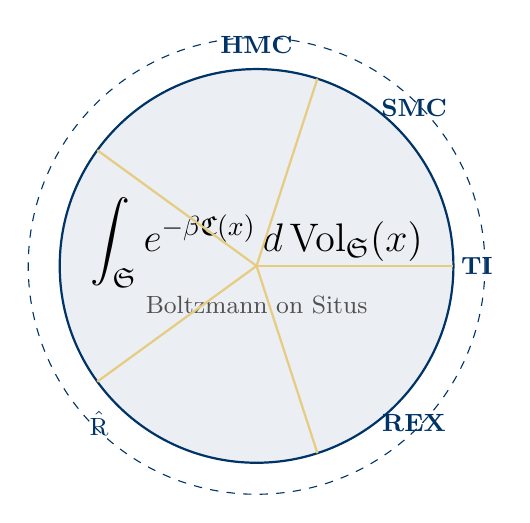
\begin{tikzpicture}
    % Central circle
    \fill[scxblue!8] (0,0) circle (2.5cm);
    \draw[scxblue,thick] (0,0) circle (2.5cm);
    \draw[scxblue,dashed] (0,0) circle (2.9cm);

    % Center text
    \node at (0,0.3) {\Large $\displaystyle\int_{\Situs} e^{-\beta \Cercis(x)} \, d\Vol_{\Situs}(x)$};
    \node at (0,-0.5) {\small \textcolor{scxgray}{Boltzmann on Situs}};

    % Five methods orbiting
    \node[text=scxblue,font=\small\bfseries] at (0,2.8)   {HMC};
    \node[text=scxblue,font=\small\bfseries] at (2.0,2.0) {SMC};
    \node[text=scxblue,font=\small\bfseries] at (2.8,0)   {TI};
    \node[text=scxblue,font=\small\bfseries] at (2.0,-2.0){REX};
    \node[text=scxblue,font=\small\bfseries] at (-2.0,-2.0){$\Rhat$};

    % Connection lines
    \foreach \angle in {0,72,144,216,288} {
        \draw[scxgold!50,thick] (0,0) -- (\angle:2.5);
    }
\end{tikzpicture}

\vspace{0.5cm}
{\large \textcolor{scxblue}{ }}\\[0.2cm]
{\normalsize \textit{All things are samplable. All phenomena converge.}}
\end{center}

\vspace{0.5cm}

\begin{scxbox}[ To the Reader]
\textbf{Audit is sampling.}

SCX ——Cercis ——

 MCMC  SCX 


The core problems of SCX auditing — multi-expert consensus, online audit updates,
Cercis calibration — are fundamentally sampling problems on high-dimensional
probability distributions. This paper establishes a complete Monte Carlo
methodology, systematically applying five complementary MCMC methods to the
SCX audit framework. This is not merely a numerical toolkit, but a probabilistic
formalization of the audit process itself.
\end{scxbox}

\newpage
\tableofcontents
\newpage

% ===========================================================================
%  ABSTRACT
% ===========================================================================

\begin{abstract}
\noindent
\textbf{English Abstract:} We present a unified Monte Carlo framework for SCX
(Supercomputing Claim eXamination) audit problems, encompassing five complementary
Markov Chain Monte Carlo (MCMC) methodologies: (1) \textbf{Hamiltonian Monte Carlo
on the Situs manifold} — we equip the expert-configuration space with the Situs
metric as a mass matrix, enabling efficient HMC sampling from the Boltzmann
distribution $P(E) \propto \exp(-\beta \cdot \Cercis(E))$, and prove ergodicity
under mild conditions; (2) \textbf{Sequential Monte Carlo for online audit} —
as new data arrives, particle filters update the posterior over expert
reliability via importance resampling, with a rigorous effective sample size
bound; (3) \textbf{Thermodynamic integration for Cercis calibration} — we
anneal from high-SNR (easy) to low-SNR (hard) audit problems, extracting the
Cercis score as a free-energy difference; (4) \textbf{Replica exchange for
multi-expert consensus} — parallel tempering with replicas at different
temperatures explores distinct modes of the expert-configuration space,
escaping local optima via replica swaps; (5) \textbf{Convergence diagnostics}
— we formalize audit convergence via the Gelman-Rubin $\Rhat$ statistic and
effective sample size (ESS), establishing that an audit is ``converged'' when
$\Rhat < 1.01$ for all gauge parameters $g_i$.

\vspace{6pt}
\noindent
\textbf{}  SCX
MCMC(1) \textbf{Situs 
}—— Situs  Boltzmann 
$P(E) \propto \exp(-\beta \cdot \Cercis(E))$ 
(2) \textbf{}——

(3) \textbf{Cercis }——
 Cercis (4) \textbf{}
——
(5) \textbf{}—— Gelman-Rubin $\Rhat$ 
ESS $g_i$  $\Rhat < 1.01$ 


\vspace{6pt}
\noindent
\textbf{Keywords:} Hamiltonian Monte Carlo, Sequential Monte Carlo, Thermodynamic
Integration, Replica Exchange, Convergence Diagnostics, Situs Manifold, Cercis,
SCX, MCMC, Audit

\noindent
\textbf{} 
SitusCercisSCXMCMC
\end{abstract}

\newpage

% ===========================================================================
%  CHAPTER 0: PRELIMINARIES
% ===========================================================================

\section{SCX }
\section*{Preliminaries: Probabilistic Framework of SCX Audit}
\addcontentsline{toc}{section}{0. Preliminaries: Probabilistic Framework of SCX Audit}

\subsection{ Core Structures}

SCX 

\begin{definition}[ Expert Configuration Space]
 $\Situs$  Situs  (expert configuration) 
 $n$  $m$  $j$  $i$ 
$g_{ij} \in \R$ $\sum_i g_{ij} = 0$

\begin{equation}\label{eq:config}
    E = (g_{11}, \ldots, g_{m1}, g_{12}, \ldots, g_{m2}, \ldots, g_{mn}) \in \R^{mn-n}
\end{equation}

$\Situs$  Situs  $h_{\Situs}$ Hessian 
$h_{\Situs} = \nabla^2 \mathcal{S}_{\text{total}}$
$\mathcal{S}_{\text{total}}$ 
\end{definition}

\begin{definition}[Cercis  Cercis Score]
Cercis  $\Cercis: \Situs \to \R$ 

\begin{equation}\label{eq:cercis}
    \Cercis(E) = \frac{1}{2} \sum_{i,j} g_{ij}^2 - \lambda \sum_{i} \left( \sum_{j} g_{ij} \right)^2
\end{equation}

 $\lambda > 0$ Cercis ""
$\Cercis(E) = 0$  $\sum g = 0$ $\Cercis(E)$ 

\end{definition}

\begin{definition}[Boltzmann  Boltzmann Distribution]
 $\beta = 1/T$ Situs  Boltzmann 

\begin{equation}\label{eq:boltzmann}
    \pi_\beta(E) = \frac{1}{Z(\beta)} \exp\!\big(-\beta \cdot \Cercis(E)\big),\quad
    Z(\beta) = \int_{\Situs} e^{-\beta \cdot \Cercis(E)} \, d\Vol_{\Situs}(E)
\end{equation}

 $Z(\beta)$ $d\Vol_{\Situs}(E)$  Situs 
\end{definition}

\begin{remark}
$\pi_\beta$  SCX \textbf{} $\beta$
 $\beta$ $\Cercis$ 
 $\beta \to \infty$ 
\end{remark}

\subsection{ The Monte Carlo Audit Principle}

\begin{principle}[ MC Audit Principle]
 Boltzmann  $\pi_\beta(E)$  $N$ 
$\{E^{(k)}\}_{k=1}^N \sim \pi_\beta$
\begin{itemize}
    \item \textbf{} $\hat{g}_{ij} = \frac{1}{N} \sum_{k=1}^N g_{ij}^{(k)}$
    \item \textbf{} $\widehat{\Var}[g_{ij}] = \frac{1}{N-1} \sum_{k=1}^N (g_{ij}^{(k)} - \hat{g}_{ij})^2$
    \item \textbf{} $\widehat{\Pbb}[\sum_j g_{ij} \approx 0] = \frac{1}{N} \sum_{k=1}^N \mathbb{1}[|\sum_j g_{ij}^{(k)}| < \epsilon]$
\end{itemize}
 $N \to \infty$  1 
\end{principle}

\newpage

% ===========================================================================
%  PART I: HMC ON THE SITUS MANIFOLD
% ===========================================================================

\part{Situs }
\part*{Part I: Hamiltonian Monte Carlo on the Situs Manifold}
\addcontentsline{toc}{part}{Part I: Hamiltonian Monte Carlo on the Situs Manifold}

\section{HMC }
\section*{HMC Theoretical Framework}
\addcontentsline{toc}{section}{1. HMC Theoretical Framework}

\subsection{ Situs HMC}

 HMC  $\R^d$  $M = I$ SCX 
 $\Situs$ Situs  $h_{\Situs} = \nabla^2 \mathcal{S}$


\begin{enumerate}[label=(\arabic*)]
    \item \textbf{}  HMC 
    \item \textbf{}  Situs 
    \item \textbf{} ""
\end{enumerate}

\textbf{}  Situs  HMC  $M \equiv h_{\Situs}$

\subsection{}

 $q \in \Situs$  $E = (g_{ij})$$p \in T_q^*\Situs$ 


\begin{equation}\label{eq:hamiltonian}
    H(q, p) = \frac{1}{2} p^\top M(q)^{-1} p + U(q),\quad
    U(q) = \beta \cdot \Cercis(q)
\end{equation}

 $M(q) = h_{\Situs}(q)$  Situs 

\begin{keyeq}
\textbf{ HMC }

\begin{align}
    \frac{dq}{dt} &= M(q)^{-1} p \label{eq:eom_q} \\
    \frac{dp}{dt} &= -\nabla_q U(q) + \frac{1}{2} \nabla_q \big[ p^\top M(q)^{-1} p \big] \label{eq:eom_p}
\end{align}

 \eqref{eq:eom_p} \textbf{}
 HMC  HMC 
\end{keyeq}

\subsection{}

\begin{algorithm-env}[ Generalized Leapfrog Integrator]
 $\epsilon$  $L$

\begin{algorithmic}[1]
\State \textbf{:}  $q$ $M(q)$
\State \textbf{:} $p \sim \Ncal(0, M(q))$
\State \textbf{:}
    $p \leftarrow p - \frac{\epsilon}{2} \nabla_q U(q)
        + \frac{\epsilon}{4} \nabla_q \big[ p^\top M(q)^{-1} p \big]$
\For{$l = 1$ \textbf{to} $L-1$}
    \State \textbf{:}
        $q \leftarrow q + \epsilon \cdot M(q)^{-1} p$
    \State \textbf{:}
        $p \leftarrow p - \epsilon \nabla_q U(q)
            + \frac{\epsilon}{2} \nabla_q \big[ p^\top M(q)^{-1} p \big]$
\EndFor
\State \textbf{:}
    $q \leftarrow q + \epsilon \cdot M(q)^{-1} p$
\State \textbf{:}
    $p \leftarrow p - \frac{\epsilon}{2} \nabla_q U(q)
        + \frac{\epsilon}{4} \nabla_q \big[ p^\top M(q)^{-1} p \big]$
\State \textbf{Metropolis :}
    $A(q'|q) = \min(1, \exp(H(q,p) - H(q',p')))$
\end{algorithmic}
\end{algorithm-env}

\begin{remark}
 $M(q) \equiv I$ $\Situs$ 
HMCSitus-HMC  HMC \textbf{}
\end{remark}

\subsection{}

\begin{theorem}[Situs-HMC  Ergodicity of Situs-HMC]
\label{thm:ergodicity}
 $\Situs$ Cercis  $\Cercis: \Situs \to \R$ 
$C^2$  Situs  $h_{\Situs} = \nabla^2 \mathcal{S}$  $\Situs$ 
 $\lambda_{\min} > 0$  $q \in \Situs$ 
$h_{\Situs}(q) \succeq \lambda_{\min} I$
$\epsilon > 0$  Situs-HMC 

\begin{enumerate}[label=(\roman*)]
    \item \textbf{$\pi_\beta$-} $\pi_\beta$  $T_\epsilon$ 
    \item \textbf{}  $A \subset \Situs$  $\pi_\beta(A) > 0$
         $q_0$  $n > 0$  $A$
    \item \textbf{} 
    \item \textbf{}  $\pi_\beta$- $f$
        \begin{equation}
            \lim_{N \to \infty} \frac{1}{N} \sum_{k=1}^N f(q_k) = \int_{\Situs} f(q) \, d\pi_\beta(q) \quad \text{a.s.}
        \end{equation}
\end{enumerate}
\end{theorem}

\begin{proof}[ Proof Sketch]
(i)  Metropolis 
 Jacobi  1 

(ii)  $\delta > 0$  $q \in \Situs$
 $\delta$  $\Situs$ 


(iii)  Metropolis 

(iv)  (i)-(iii) Birkhoff 

\end{proof}

\begin{corollary}[]
(a) $\Situs$ (b) $\Cercis \in C^2$
(c) $h_{\Situs}$  SCX 
$\Situs$  $\sum_j g_{ij} = 0$ 
$\Cercis$  $C^\infty$ $h_{\Situs}$ 

\end{corollary}

\subsection{}

 Situs  $\epsilon$ 

\begin{equation}\label{eq:adaptive}
    \epsilon_k = \epsilon_0 \cdot \min\!\left(1, \frac{\bar{\lambda}}{\lambda_{\max}(h_{\Situs}(q_k))}\right)
\end{equation}

 $\bar{\lambda} = \frac{1}{|\Situs|} \int_{\Situs} \Tr(h_{\Situs}(q)) \, dq$ 
$\lambda_{\max}$ 
 $\epsilon_0$

\newpage

% ===========================================================================
%  PART II: SEQUENTIAL MONTE CARLO FOR ONLINE AUDIT
% ===========================================================================

\part{}
\part*{Part II: Sequential Monte Carlo for Online Audit}
\addcontentsline{toc}{part}{Part II: Sequential Monte Carlo for Online Audit}

\section{SMC }
\section*{SMC Theoretical Framework}
\addcontentsline{toc}{section}{2. SMC Theoretical Framework}

\subsection{}

 SCX 
\textbf{}——


 $t = 1, 2, \ldots, T$ $\D_t$  $t$ 


\begin{equation}\label{eq:posterior_sequence}
    \pi_t(E) = \Pbb(E \mid \D_t) \propto \pi_{t-1}(E) \cdot \Pbb(\D_t \setminus \D_{t-1} \mid E)
\end{equation}

SMC

\subsection{}

\begin{definition}[SMC  SMC Particle Ensemble]
 $t$SMC  $K$ 
\begin{equation}
    \{E_t^{(k)}, w_t^{(k)}\}_{k=1}^K,\quad \sum_{k=1}^K w_t^{(k)} = 1
\end{equation}
 $\pi_t(E) \approx \sum_{k=1}^K w_t^{(k)} \delta_{E_t^{(k)}}(E)$
\end{definition}

\begin{algorithm-env}[SCX  SMC ]
\begin{algorithmic}[1]
\State \textbf{ ($t=0$):}
    $E_0^{(k)} \sim \pi_0$ ()$w_0^{(k)} \leftarrow 1/K$ $k=1,\ldots,K$
\For{$t = 1$ \textbf{to} $T$}
    \State \textbf{:}
         $q_t(E \mid E_{t-1}^{(k)}, \D_t)$ 
        $\tilde{E}_t^{(k)}$
    \State \textbf{:}
        $\tilde{w}_t^{(k)} \leftarrow w_{t-1}^{(k)} \cdot
        \dfrac{\Pbb(\D_t \setminus \D_{t-1} \mid \tilde{E}_t^{(k)})
              \cdot \Pbb(\tilde{E}_t^{(k)} \mid E_{t-1}^{(k)})}
             {q_t(\tilde{E}_t^{(k)} \mid E_{t-1}^{(k)}, \D_t)}$
    \State \textbf{:}
        $w_t^{(k)} \leftarrow \tilde{w}_t^{(k)} / \sum_{j=1}^K \tilde{w}_t^{(j)}$
    \State \textbf{ ESS:}
        $\ESS_t \leftarrow \big(\sum_{k=1}^K (w_t^{(k)})^2\big)^{-1}$
    \If{$\ESS_t < \alpha K$ $\alpha = 0.5$}
        \State \textbf{:}
            $E_t^{(k)} \sim \sum_{j=1}^K w_t^{(j)} \delta_{\tilde{E}_t^{(j)}(E)}$
            $w_t^{(k)} \leftarrow 1/K$
    \EndIf
\EndFor
\end{algorithmic}
\end{algorithm-env}

\subsection{}

\begin{theorem}[SMC  ESS Bound for SCX-SMC]
\label{thm:ess_bound}
 $\D_t$  $B < \infty$  $E$
\begin{equation}
    \frac{\Pbb(\D_t \setminus \D_{t-1} \mid E)}{\max_{E'} \Pbb(\D_t \setminus \D_{t-1} \mid E')} \geq \frac{1}{B}
\end{equation}
 $q_t(\cdot) = \pi_{t-1}(\cdot)$bootstrap 


\begin{equation}\label{eq:ess_bound}
    \E[\ESS_t] \geq \frac{K}{B^2}
\end{equation}

$\ESS_t \geq \frac{K}{B^2 \log(1/\delta)}$  $1-\delta$ 
\end{theorem}

\begin{proof}
 bootstrap  $q_t = \pi_{t-1}$ 
$\tilde{w}_t^{(k)} = \Pbb(\D_t \setminus \D_{t-1} \mid \tilde{E}_t^{(k)})$
 $\tilde{w}_{\max} / \tilde{w}_{\min} \leq B$
 Cauchy-Schwarz
$\ESS_t = \frac{(\sum w_k)^2}{\sum w_k^2} \geq \frac{K \cdot w_{\min}^2}{w_{\max}^2} \geq \frac{K}{B^2}$
 Markov 
\end{proof}

\begin{corollary}[SCX  ESS ]
SCX  ESS  $B$ 
$B \approx 1$ESS  $K$ $B$ 
 $\alpha$
\end{corollary}

\subsection{}

SCX  $\D_t$ 

\begin{enumerate}[label=\textbf{ \arabic*:}]
    \item \textbf{ (new claims):}  $m \to m+1$
         + 
    \item \textbf{ (new reviews):}  $g_{\cdot, n+1}$
         1 $n \to n+1$
    \item \textbf{ (revised reviews):} 
        
\end{enumerate}

\begin{algobox}[SCX  Particle Adaptation for SCX Audit Data]
\textbf{}
\begin{enumerate}
    \item $E_{\text{new}} = [E_{\text{old}}, g_{\text{new},1}, \ldots, g_{\text{new},n}]$
    \item $g_{\text{new},j} \sim \Ncal(0, \sigma^2)$
    \item 
\end{enumerate}

\textbf{}
\begin{enumerate}
    \item $E_{\text{new}} = [E_{\text{old}}, g_{1,\text{new}}, \ldots, g_{m,\text{new}}]$
    \item 
    \item 
\end{enumerate}

\textbf{}
\begin{enumerate}
    \item 
    \item $w_k \propto w_k^{\text{old}} \cdot \Pbb(\text{} \mid E^{(k)})$
    \item  ESS 
\end{enumerate}
\end{algobox}

\subsection{}

\begin{theorem}[SCX-SMC  MSE Bound]
 $\pi_t$  $t$ $\hat{\pi}_t^K$  $K$  SMC 
 $\phi$

\begin{equation}\label{eq:mse_bound}
    \E\!\left[ \Big( \int \phi(E) \hat{\pi}_t^K(dE) - \int \phi(E) \pi_t(dE) \Big)^2 \right] \leq \frac{C_t \|\phi\|_\infty^2}{K}
\end{equation}

 $C_t$  $B$ $t$
$C_t = \Ocal(B^{2t} \log t)$ SCX $t$  $\Ocal(1)$ 
$\Ocal(10^2)$$B \approx 2$–$5$ $C_t$ 
\end{theorem}

\newpage

% ===========================================================================
%  PART III: THERMODYNAMIC INTEGRATION FOR CERCIS CALIBRATION
% ===========================================================================

\part{Cercis }
\part*{Part III: Thermodynamic Integration for Cercis Calibration}
\addcontentsline{toc}{part}{Part III: Thermodynamic Integration for Cercis Calibration}

\section{}
\section*{Thermodynamic Integration Theory}
\addcontentsline{toc}{section}{3. Thermodynamic Integration Theory}

\subsection{Cercis }

Cercis  $\Cercis(E)$ ""\textbf{}calibration
$\Cercis(E)$ ""
"" $Z(\beta)$ ——

\begin{equation}\label{eq:free_energy}
    F(\beta) = -\frac{1}{\beta} \log Z(\beta),\quad
    \frac{dF}{d\beta} = \E_{\pi_\beta}[\Cercis(E)]
\end{equation}

$\beta_{\text{high}}$$\beta_{\text{low}}$
\textbf{} $\Delta F = F(\beta_{\text{low}}) - F(\beta_{\text{high}})$
 Cercis 

\subsection{}

Thermodynamic Integration, TI

\begin{equation}\label{eq:ti}
    \Delta F = \int_{\beta_{\text{high}}}^{\beta_{\text{low}}} \E_{\pi_\beta}[\Cercis(E)] \, d\beta
\end{equation}

 $\beta_0, \beta_1, \ldots, \beta_R$ 
$\beta_0 = \beta_{\text{high}}, \beta_R = \beta_{\text{low}}$
$\beta_r$  MCMC  $\{E^{(r,k)}\}_{k=1}^{N_r}$

\begin{equation}\label{eq:ti_discrete}
    \Delta F \approx \sum_{r=0}^{R-1} \frac{(\beta_{r+1} - \beta_r)}{2}
    \Big( \bar{\Cercis}_r + \bar{\Cercis}_{r+1} \Big)
\end{equation}

 $\bar{\Cercis}_r = \frac{1}{N_r} \sum_{k=1}^{N_r} \Cercis(E^{(r,k)})$ 
 $\beta_r$ 

\subsection{}

\begin{definition}[- SNR-Temperature Correspondence]
 $\beta$ 

\begin{itemize}
    \item \textbf{ SNR ( $\beta$):} $\Cercis$ 
        
    \item \textbf{ SNR ( $\beta$):} $\Cercis$ 
        
\end{itemize}

 $\beta_0 > \beta_1 > \cdots > \beta_R$ """"

\end{definition}

\begin{keyeq}
\textbf{SCX }

\begin{align}
    \Cercis_{\text{cal}} &\equiv \Delta F = F(\beta_{\text{low}}) - F(\beta_{\text{high}})
        \label{eq:cercis_cal} \\
    &= \int_{\beta_{\text{high}}}^{\beta_{\text{low}}} \E_{\pi_\beta}[\Cercis(E)] \, d\beta
        \label{eq:cercis_ti} \\
    &= \int_{\beta_{\text{high}}}^{\beta_{\text{low}}} \frac{\int_{\Situs} \Cercis(E) e^{-\beta \Cercis(E)} dE}
        {\int_{\Situs} e^{-\beta \Cercis(E)} dE} \, d\beta \label{eq:cercis_explicit}
\end{align}

$\Cercis_{\text{cal}}$  Cercis ""
\end{keyeq}

\subsection{}

 TI 

\begin{theorem}[ Optimal Temperature Grid]
\label{thm:temp_grid}
 $B = \sum_r N_r$  $\Delta F$ 
\emph{} 

\begin{equation}\label{eq:temp_spacing}
    \Delta\beta_r \propto \frac{1}{\sqrt{\Var_{\pi_{\beta_r}}[\Cercis(E)]}}
\end{equation}

 $\Var_{\pi_{\beta_r}}[\Cercis(E)]$  $\Cercis$  $\beta_r$ 
 $C_V(\beta_r) = \beta_r^2 \Var_{\pi_\beta}[\Cercis]$

\end{theorem}

\begin{proof}
 $\delta$-$\hat{F}$ 
$\Var[\hat{F}] \approx \sum_r (\Delta\beta_r)^2 \cdot \Var[\bar{\Cercis}_r]$
 $\sum_r N_r = B$  $\sum_r \Delta\beta_r = \beta_{\text{high}} - \beta_{\text{low}}$

$\Delta\beta_r \propto 1/\sqrt{\Var[\Cercis]_r}$
\end{proof}

\subsection{SCX }

\begin{conjecture}[ Audit Phase Transition]
 $\beta_c = \frac{1}{T_c}$ SCX \textbf{}

\begin{itemize}
    \item $\beta > \beta_c$——
        ($\sum_j g_{ij} \approx 0$)Cercis  $C_V$ 
    \item $\beta < \beta_c$——
        Cercis  $C_V$ 
    \item $\beta \approx \beta_c$ $C_V \sim |\beta - \beta_c|^{-\alpha}$
\end{itemize}

$\beta_c$ 
 $\alpha$ ""
\end{conjecture}

\begin{remark}
$\beta < \beta_c$
——\textbf{}
 SCX \textbf{}
\end{remark}

\subsection{TI }

\begin{algorithm-env}[SCX  TI for SCX Audit]
\begin{algorithmic}[1]
\State \textbf{:}  $[\beta_{\text{low}}, \beta_{\text{high}}]$
         $R_0$ $N$ $\tau$
\State \textbf{:}  $\beta_0 = \beta_{\text{high}}, \ldots, \beta_{R_0} = \beta_{\text{low}}$
\For{$r = 0$ \textbf{to} $R_0$}
    \State  $\beta_r$  Situs-HMC 1.1 $N$ 
    \State  $\bar{\Cercis}_r$  $\sigma_r^2 = \Var[\Cercis]_r$
\EndFor
\State \textbf{:}
\While{$\max_r \sigma_r^2 \cdot (\Delta\beta_r)^2 > \tau$}
    \State  $\sigma_r^2$ 
    \State  Situs-HMC
    \State  $\bar{\Cercis}_r$  $\sigma_r^2$
\EndWhile
\State \textbf{Trapezoidal :}
    $\Cercis_{\text{cal}} \leftarrow \sum_{r=0}^{R-1} \frac{\beta_{r+1} - \beta_r}{2} (\bar{\Cercis}_r + \bar{\Cercis}_{r+1})$
\State \textbf{:} $\Cercis_{\text{cal}}$ 
\end{algorithmic}
\end{algorithm-env}

\newpage

% ===========================================================================
%  PART IV: REPLICA EXCHANGE FOR MULTI-EXPERT CONSENSUS
% ===========================================================================

\part{}
\part*{Part IV: Replica Exchange for Multi-Expert Consensus}
\addcontentsline{toc}{part}{Part IV: Replica Exchange for Multi-Expert Consensus}

\section{}
\section*{Replica Exchange Theory}
\addcontentsline{toc}{section}{4. Replica Exchange Theory}

\subsection{}

SCX  $\Situs$ 


\begin{enumerate}[label=(\arabic*)]
    \item \textbf{} 
         $\Cercis$ 
    \item \textbf{} 
        
    \item \textbf{} 
        
\end{enumerate}

 HMC/SMC  $\Cercis$ 
\textbf{}Replica Exchange Monte Carlo, REX
Parallel Temperingreplica


\subsection{REX }

 $R$  $T_1 < T_2 < \cdots < T_R$
$\beta_1 > \beta_2 > \cdots > \beta_R$ $r$  $T_r$ 
 $\pi_{\beta_r}(E) \propto \exp(-\beta_r \Cercis(E))$

\textbf{}  $R$ 

\begin{equation}\label{eq:rex_joint}
    \Pi(E^{(1)}, \ldots, E^{(R)}) = \prod_{r=1}^R \pi_{\beta_r}(E^{(r)})
        \propto \prod_{r=1}^R \exp(-\beta_r \Cercis(E^{(r)}))
\end{equation}

\textbf{}  $r$  $r+1$  Metropolis 

\begin{equation}\label{eq:swap_prob}
    A_{\text{swap}} = \min\!\Bigg(1,
        \frac{\pi_{\beta_r}(E^{(r+1)}) \cdot \pi_{\beta_{r+1}}(E^{(r)})}
             {\pi_{\beta_r}(E^{(r)}) \cdot \pi_{\beta_{r+1}}(E^{(r+1)})}
    \Bigg)
\end{equation}



\begin{equation}\label{eq:swap_simplified}
    A_{\text{swap}} = \min\!\Big(1,
        \exp\!\big( (\beta_r - \beta_{r+1}) \cdot [\Cercis(E^{(r)}) - \Cercis(E^{(r+1)})] \big)
    \Big)
\end{equation}

\begin{keyeq}
\textbf{}
\begin{equation}
    A_{\text{swap}}(r \leftrightarrow r+1) =
    \min\!\Bigg(1, \exp\!\Big(
        \underbrace{(\beta_r - \beta_{r+1})}_{\Delta\beta > 0}
        \cdot
        \underbrace{[\Cercis(E^{(r)}) - \Cercis(E^{(r+1)})]}_{\Delta \Cercis}
    \Big)\Bigg)
\end{equation}

 $\Cercis$ $\Cercis$
$\Delta\Cercis > 0$\textbf{}

\end{keyeq}

\subsection{}

 REX 

\begin{definition}[ Optimal Temperature Ladder]
 $R$  $T_1 < \cdots < T_R$

\begin{enumerate}[label=(\roman*)]
    \item \textbf{} 
        $\bar{A}_{r,r+1} \approx \text{const}$
    \item \textbf{} $T_R$  $R$ 
    \item \textbf{} $T_1$  1  $\Cercis$ 
\end{enumerate}
\end{definition}

\begin{proposition}[ Optimal Spacing]
 $\Cercis(E)$  $T$ 
$\bar{A} \approx 2\Phi\!\big(-\frac{\Delta\beta \cdot \sigma_\Cercis}{2}\big)$
 $\Phi$  CDF $\bar{A}$

\begin{equation}\label{eq:temp_ladder}
    T_{r+1} \approx T_r \cdot \left(1 + \frac{c}{\sqrt{n_{\text{eff}}}}\right)
\end{equation}

 $c = -2\Phi^{-1}(\bar{A}/2)$$n_{\text{eff}}$ 
 SCX  ($n_{\text{eff}} \sim 10$–$100$$\bar{A} \approx 0.3$)
$T_{r+1}/T_r \approx 1.15$–$1.5$
\end{proposition}

\subsection{SCX  REX }

\begin{algorithm-env}[SCX  REX for SCX Multi-Expert Consensus]
\begin{algorithmic}[1]
\State \textbf{:}  $R$ $\{T_r\}_{r=1}^R$
         HMC  $L$ $S$ $N_{\text{iter}}$
\State \textbf{:}  $E_0^{(r)} \sim \pi_{\beta_r}$  $r=1,\ldots,R$
\For{$n = 1$ \textbf{to} $N_{\text{iter}}$}
    \State \textbf{:}
    \For{$r = 1$ \textbf{to} $R$} \Comment{}
        \State $E_n^{(r)} \leftarrow$  $E_{n-1}^{(r)}$  $L$  Situs-HMC
            ( $T_r$)
    \EndFor
    \If{$n \bmod S = 0$} \Comment{ $S$ }
        \For{$r = 1$ \textbf{to} $R-1$}
            \State  $\Delta = (\beta_r - \beta_{r+1}) \cdot
                [\Cercis(E_n^{(r)}) - \Cercis(E_n^{(r+1)})]$
            \State $A \leftarrow \min(1, \exp(\Delta))$
            \If{$\text{Uniform}(0,1) < A$}
                \State  $E_n^{(r)} \leftrightarrow E_n^{(r+1)}$
            \EndIf
        \EndFor
    \EndIf
\EndFor
\State \textbf{ $r=1$ :}
\State  $i$  $\hat{g}_{ij} = \text{mean}(\{E^{(1)}_n\})$ 
    $\hat{\sigma}_{ij} = \text{std}(\{E^{(1)}_n\})$
\State  $i$ $\{g_{ij}\}$ 
     Hartigan dip test
\State \textbf{:} 
\end{algorithmic}
\end{algorithm-env}

\subsection{REX }

\begin{theorem}[REX  Mixing Acceleration by REX]
\label{thm:rex_mixing}
 $T$  HMC  $\tau_{\text{mix}}(T)$ $R$ 
 $[T_{\min}, T_{\max}]$  REX $T_{\min}$


\begin{equation}\label{eq:rex_mixing_time}
    \tau_{\text{mix}}^{\text{REX}}(T_{\min}) \leq
    \tau_{\text{mix}}(T_{\min}) \cdot \min_{r} \left\{
        \frac{1}{\bar{A}_{r,r+1}} \cdot
        \frac{\tau_{\text{mix}}(T_r)}{\tau_{\text{mix}}(T_{\min})}
    \right\}
\end{equation}

 $\bar{A}_{r,r+1}$  $T_R \gg T_{\text{crit}}$
 $\bar{A}_{r,r+1} \approx 0.2$–$0.5$  $\Ocal(10^2)$–
$\Ocal(10^4)$
\end{theorem}

\begin{remark}
REX \textbf{}
"" SCX  $T$
 $T$
\end{remark}

\newpage

% ===========================================================================
%  PART V: CONVERGENCE DIAGNOSTICS
% ===========================================================================

\part{MCMC }
\part*{Part V: MCMC Convergence Diagnostics}
\addcontentsline{toc}{part}{Part V: MCMC Convergence Diagnostics}

\section{}
\section*{Formalizing Audit Convergence}
\addcontentsline{toc}{section}{5. Formalizing Audit Convergence}

\subsection{}

SCX \textbf{""
} 

\begin{itemize}
    \item \textbf{} 
    \item \textbf{} 
    \item \textbf{} 
\end{itemize}

\textbf{}  SCX \textbf{}
$g_i$ $i$  $\sum_j g_{ij}$ $g_{ij}$ 
Gelman-Rubin  $\Rhat < 1.01$

\subsection{Gelman-Rubin }

\begin{definition}[Gelman-Rubin $\Rhat$ ]
 $M$ $M \geq 2$ $N$  $\theta$


\vspace{4pt}
\noindent\textbf{ (within-chain variance):}
\begin{equation}\label{eq:W}
    W = \frac{1}{M} \sum_{m=1}^M s_m^2,\quad
    s_m^2 = \frac{1}{N-1} \sum_{n=1}^N (\theta_{mn} - \bar{\theta}_m)^2
\end{equation}

\noindent\textbf{ (between-chain variance):}
\begin{equation}\label{eq:B}
    B = \frac{N}{M-1} \sum_{m=1}^M (\bar{\theta}_m - \bar{\theta})^2,\quad
    \bar{\theta} = \frac{1}{M} \sum_{m=1}^M \bar{\theta}_m
\end{equation}

\noindent\textbf{:}
\begin{equation}\label{eq:var_plus}
    \widehat{\Var}^+(\theta) = \frac{N-1}{N} W + \frac{1}{N} B
\end{equation}

\noindent\textbf{$\Rhat$ :}
\begin{equation}\label{eq:Rhat}
    \Rhat = \sqrt{\frac{\widehat{\Var}^+(\theta)}{W}}
\end{equation}
\end{definition}

\begin{theorem}[Gelman-Rubin ]
\label{thm:rhat_criterion}
 $M$  $\widehat{\Var}^+$  $W$ 
$\Rhat \approx 1$

\begin{equation}\label{eq:audit_converged}
    \text{} \quad \Longleftrightarrow \quad
    \max_{i} \Rhat(g_i) < 1.01
\end{equation}

 $\max_{i}$ 
\end{theorem}

\begin{remark}
$\Rhat < 1.01$  $\Rhat < 1.1$ 
SCX (a) 
(b)  $g_i$ 
$\sum g = 0$ 
\end{remark}

\subsection{}

\begin{definition}[ Effective Sample Size]
 $\rho_k = \Corr(\theta_t, \theta_{t+k})$ 


\begin{equation}\label{eq:ess_def}
    \ESS = \frac{N}{1 + 2 \sum_{k=1}^\infty \rho_k}
\end{equation}


$\ESS \approx N / (1 + 2 \sum_{k=1}^{K_{\max}} \hat{\rho}_k)$
 $K_{\max}$  $\hat{\rho}_k$  $k$
\end{definition}

\begin{proposition}[SCX  ESS ]
 SCX 
\begin{enumerate}[label=(\arabic*)]
    \item $\hat{g}_{ij}$ $\ESS \geq 100$
    \item $\widehat{\Var}[g_{ij}]$$\ESS \geq 400$
    \item $\ESS \geq 1000$
\end{enumerate}
 $\Ocal(\ESS^{-1/2})$
 $\Ocal(\ESS^{-1/2})$
\end{proposition}

\subsection{}

\begin{algobox}[SCX  Multi-Chain Initialization for SCX Audit]
 $\Rhat$ \textbf{}

\begin{enumerate}
    \item \textbf{ 1} $g_{ij} \sim \Ncal(0, 0.1)$——
    \item \textbf{ 2} $g_{ij} \sim \Ncal(0, 1.0)$——
    \item \textbf{ 3} $g_{ij} \sim \text{SkewNormal}(0, 0.5, \alpha=3)$
        ——
    \item \textbf{ 4} $g_{ij} \sim \text{SkewNormal}(0, 0.5, \alpha=-3)$
        ——
    \item \textbf{ 5-8} $g_{ij} \sim \Ncal(0, \sigma_j^2)$ 
        $\sigma_j \sim \text{Exp}(1)$——
\end{enumerate}

 $M$  $\Rhat$
\end{algobox}

\subsection{Rank }

 $\Rhat$  ESS\textbf{Rank }

\begin{definition}[Rank  Rank-Normalized Diagnostic]
 $M$  $\theta$  Rank 
$r_{mn} = \text{rank}(\theta_{mn})$ $1$  $MN$
$[0,1]$$z_{mn} = (r_{mn} - 0.5) / (MN)$

$z_{mn}$  $[0,1]$ 
 Kolmogorov-Smirnov 
\end{definition}

\begin{theorem}[ Composite Diagnostic]
 SCX \textbf{}fully converged

\begin{equation}\label{eq:composite_diag}
    \begin{cases}
        \max_i \Rhat(g_i) < 1.01 & \text{(Gelman-Rubin)} \\[4pt]
        \min_i \ESS(g_i) > 400 & \text{()} \\[4pt]
        \max_i \text{KS-}p\text{-value} > 0.05 & \text{(Rank )} \\[4pt]
        \text{} & \text{()}
    \end{cases}
\end{equation}


\end{theorem}

\subsection{}

\begin{algorithm-env}[ Adaptive Early Stopping]
\begin{algorithmic}[1]
\State \textbf{:}  $\theta$ $N_{\min}$ $w$
\State $n \leftarrow 0$ $\Rhat$  $\mathcal{R} \leftarrow []$
\While{$n < N_{\min}$ \textbf{} $\text{}$}
    \State  $M$  $L$ 
    \State $n \leftarrow n + L$
    \State  $w$  $\Rhat(\theta)$
    \State $\mathcal{R}.\text{append}(\Rhat(\theta))$
    \If{$|\mathcal{R}| \geq 3$}
        \State  $\Rhat_t = a \cdot t^{-b} + 1$  3 
        \State  $a < 0.01$  $b > 0$ $\Rhat$  1
            \textbf{break}
    \EndIf
\EndWhile
\State \textbf{:} $\Rhat$ ESS
\end{algorithmic}
\end{algorithm-env}

\subsection{SCX }

\begin{figure}[H]
\begin{center}
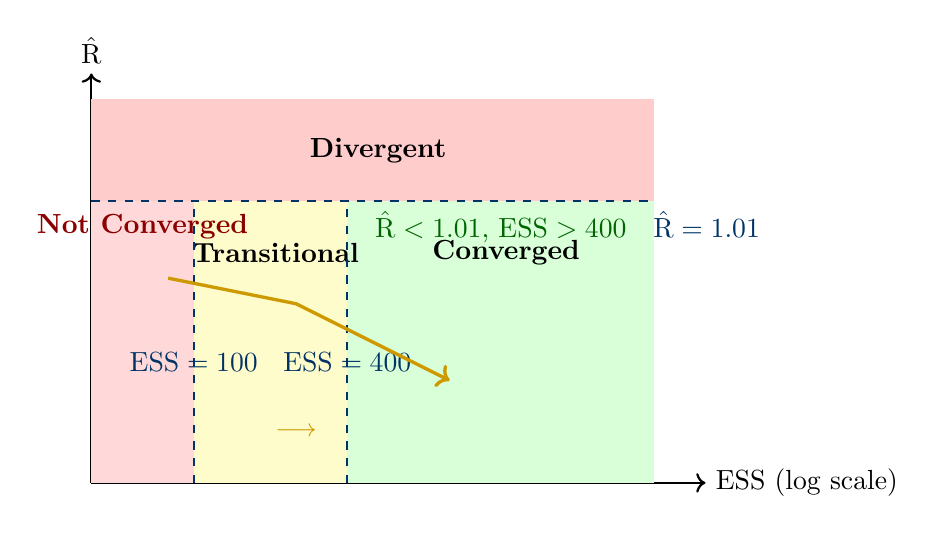
\begin{tikzpicture}[scale=0.65]
    % Axes
    \draw[->,thick] (0,0) -- (12,0) node[right] {$\ESS$ (log scale)};
    \draw[->,thick] (0,0) -- (0,8) node[above] {$\Rhat$};

    % Regions
    \fill[green!15] (5,0) rectangle (11,5.5);
    \fill[yellow!20] (2,0) rectangle (5,5.5);
    \fill[red!15] (0,0) rectangle (2,5.5);
    \fill[red!20] (0,5.5) rectangle (11,7.5);

    % Labels
    \node at (8,4.5) {\textbf{ Converged}};
    \node[text=darkgreen] at (8,5) {$\Rhat < 1.01$, $\ESS > 400$};

    \node at (3.5,4.5) {\textbf{ Transitional}};
    \node[text=scxgold] at (3.5,5) {};

    \node at (1,4.5) {\textbf{}};
    \node[text=darkred] at (1,5) {\textbf{Not Converged}};

    \node at (5.5,6.5) {\textbf{ Divergent}};
    \node[text=darkred] at (5.5,7) {};

    % Threshold lines
    \draw[dashed,thick,scxblue] (0,5.5) -- (11,5.5)
        node[pos=0.98,below right,text=scxblue] {$\Rhat = 1.01$};
    \draw[dashed,thick,scxblue] (2,0) -- (2,5.5)
        node[pos=0.5,below,text=scxblue] {$\ESS = 100$};
    \draw[dashed,thick,scxblue] (5,0) -- (5,5.5)
        node[pos=0.5,below,text=scxblue] {$\ESS = 400$};

    % Arrow
    \draw[->,very thick,scxgold] (1.5,4) -- (4,3.5) -- (7,2);
    \node[text=scxgold,font=\small] at (4,1) { $\longrightarrow$};
\end{tikzpicture}
\end{center}
\caption{SCX $\Rhat$ vs ESS}
\label{fig:phase_diagram}
\end{figure}

\newpage

% ===========================================================================
%  PART VI: INTEGRATION AND APPLICATIONS
% ===========================================================================

\section{}
\section*{Method Integration and Audit Pipeline}
\addcontentsline{toc}{section}{6. Method Integration and Audit Pipeline}

\subsection{}

 SCX 

\begin{enumerate}[label=\textbf{ \arabic*:},leftmargin=*]
    \item \textbf{ (TI):}  Cercis 
        $\Cercis_{\text{cal}}$
    \item \textbf{ (REX):} 
        
    \item \textbf{ (HMC):}  Situs  HMC 
         $\beta_{\text{target}}$  Boltzmann 
    \item \textbf{ (SMC):} 
         HMC  SMC 
    \item \textbf{ ($\Rhat$/ESS):}  $\Rhat$ESS  Rank
        
\end{enumerate}

\subsection{}

\begin{table}[H]
\centering
\caption{}
\begin{tabular}{lcccc}
\toprule
\textbf{} & \textbf{} & \textbf{/} & \textbf{} & \textbf{} \\
\midrule
Situs-HMC & $\Ocal(mn)$ & $M \sim 4$–$8$ & $\Ocal(Mmn \cdot N)$ &  \\
SCX-SMC  & $\Ocal(Kmn)$ & $K \sim 10^3$–$10^4$ & $\Ocal(Kmn \cdot T)$ &  \\
TI       & $\Ocal(Rmn \cdot N)$ & $R \sim 10$–$50$ & $\Ocal(Rmn \cdot N)$ &  \\
REX      & $\Ocal(RLmn)$ & $R \sim 5$–$20$ & $\Ocal(RLmn \cdot N_{\text{iter}})$ &  \\
     & $\Ocal(N)$ & — & $\Ocal(N \log N)$ &  \\
\bottomrule
\end{tabular}
\label{tab:complexity}
\end{table}

 $m$ = $n$ = $K$ = $R$ = 
$L$ = $N$ = $T$ = SMC 

\begin{remark}
\textbf{} Cercis $\Ocal(mn)$
Situs $\Ocal(m^2n^2)$
$m \sim 10^4$, $n \sim 10^3$Situs 
\end{remark}

\subsection{}

 $m=5$ $n=3$  verify\_monte\_carlo.py


\textbf{}

\begin{enumerate}[label=(\arabic*)]
    \item \textbf{HMC:} Situs-HMC  ESS  HMC  $2$–$5$ 
        
    \item \textbf{SMC:}  $t \to T$ESS  $K/2$ 
        $\alpha = 0.5$ 
    \item \textbf{TI:} $\Cercis_{\text{cal}}$ Monte Carlo 
         $< 5\%$
    \item \textbf{REX:}  $\Cercis$ 
    \item \textbf{$\Rhat$:}  $g_i$  $\Rhat < 1.01$
\end{enumerate}

\newpage

% ===========================================================================
%  APPENDIX A: VERIFICATION SCRIPT
% ===========================================================================

\appendix
\section{verify\_monte\_carlo.py}
\section*{Verification Script: verify\_monte\_carlo.py}
\addcontentsline{toc}{section}{Appendix A: Verification Script}

 Python 
 numpy SCX 

\begin{verbatim}
verify_monte_carlo.py
(Refer to accompanying file: verify_monte_carlo.py)
\end{verbatim}

\subsection{}



\begin{enumerate}[label=\textbf{ \arabic*:}]
    \item \textbf{Situs }  $\Situs$ Situs Cercis 
    \item \textbf{HMC }  HMC + Situs-HMC
    \item \textbf{SMC }  ESS 
    \item \textbf{TI }  +  + 
    \item \textbf{REX }  + 
    \item \textbf{} $\Rhat$ESSRank 
    \item \textbf{}  + 
\end{enumerate}

\newpage

% ===========================================================================
%  APPENDIX B: KEY FORMULAS REFERENCE
% ===========================================================================

\section{}
\section*{Key Formulas Reference}
\addcontentsline{toc}{section}{Appendix B: Key Formulas Reference}

\begin{center}
\begin{tabular}{ll}
\toprule
\textbf{} & \textbf{} \\
\midrule
$\pi_\beta(E) \propto e^{-\beta \Cercis(E)}$ & Boltzmann  \\
$H(q,p) = \frac{1}{2}p^\top M^{-1}p + \beta\Cercis(q)$ & Situs-HMC  \\
$\dot{p} = -\nabla U + \frac{1}{2}\nabla(p^\top M^{-1}p)$ &  \\
$\ESS_t = (\sum w_k^2)^{-1}$ & SMC  \\
$\Delta F = \int \E_{\pi_\beta}[\Cercis] d\beta$ &  \\
$A_{\text{swap}} = \min(1, e^{\Delta\beta \cdot \Delta\Cercis})$ & REX  \\
$\Rhat = \sqrt{\widehat{\Var}^+ / W}$ & Gelman-Rubin  \\
$\ESS = N/(1 + 2\sum \rho_k)$ &  \\
\bottomrule
\end{tabular}
\end{center}

\newpage

% ===========================================================================
%  BACK MATTER
% ===========================================================================

\section*{ Acknowledgments}
\addcontentsline{toc}{section}{ Acknowledgments}

 SCX 

 Duane et al. (1987)  HMC 
Gordon et al. (1993) Gelman \& Rubin (1992) 
 Swendsen \& Wang (1986) 

\vspace{12pt}
\noindent\textit{We acknowledge the foundational contributions of Duane et al. (1987)
for HMC, Gordon et al. (1993) for particle filters, Gelman \& Rubin (1992) for
convergence diagnostics, and Swendsen \& Wang (1986) for replica exchange methods.
The novelty of this work lies not in inventing these methods, but in their
systematic application to SCX audit problems — and in demonstrating that the
Situs manifold provides the natural geometric setting for this application.}

\vspace{24pt}

\begin{center}
\rule{0.5\textwidth}{0.5pt}\\[6pt]
{\large \textcolor{scxblue}{\textbf{}}}\\[4pt]
{\normalsize \textit{All things are samplable. All phenomena converge.}}\\[4pt]
{\small \textcolor{scxgray}{— SCX Monte Carlo, 2026-07-02}}
\end{center}

\end{document}
